%=============================================================================%
% Author: 	John Joseph Valletta, Bram Kuijper
% Date: 	23/04/2017, 27/03/2019
% Title: 	Python workshop: Matplotlib
%=============================================================================%

%=============================================================================%
% Preamble
%=============================================================================%
% Libraries
\documentclass[xcolor=table]{beamer}
\usepackage{beamerthemeshadow}
\usepackage[T1]{fontenc}
\usepackage{helvet}
\usepackage[]{graphicx}
\usepackage{array}
\usepackage{color}
\definecolor{dkgreen}{rgb}{0,0.6,0}
\definecolor{gray}{rgb}{0.5,0.5,0.5}
\definecolor{mauve}{rgb}{0.58,0,0.82}
\definecolor{deepblue}{rgb}{0,0,0.5}
\definecolor{deepred}{rgb}{0.6,0,0}
\definecolor{deepgreen}{rgb}{0,0.5,0}
\definecolor{lightgray}{rgb}{0.92,0.92,0.92}
\usepackage{listings} % to insert code
\usepackage{textpos} % textblock
\usepackage{textcomp} % textblock
\usepackage{hyperref}
\hypersetup{colorlinks=true, urlcolor=blue, linkcolor=black} 
% Listing set up
% bash
\lstdefinestyle{bash}{
language=bash,                     % the language of the code
basicstyle=\scriptsize\ttfamily,       % the size of the fonts that are used for the code
numbers=none,%left,                   % where to put the line-numbers
numberstyle=\tiny\color{gray},  % the style that is used for the line-numbers
stepnumber=1,                   % the step between two line-numbers. If it's 1, each line
                          % will be numbered
numbersep=5pt,                  % how far the line-numbers are from the code
backgroundcolor=\color{lightgray},  % choose the background color. You must add \usepackage{color}
showspaces=false,               % show spaces adding particular underscores
showstringspaces=false,         % underline spaces within strings
showtabs=false,                 % show tabs within strings adding particular underscores
frame=lines,%single,                   % adds a frame around the code
rulecolor=\color{black},        % if not set, the frame-color may be changed on line-breaks within not-black text (e.g. commens (green here))
tabsize=2,                      % sets default tabsize to 2 spaces
captionpos=b,                   % sets the caption-position to bottom
breaklines=true,                % sets automatic line breaking
breakatwhitespace=false,        % sets if automatic breaks should only happen at whitespace
title=\lstname,                 % show the filename of files included with \lstinputlisting;
                          % also try caption instead of title
keywordstyle=\color{blue},      % keyword style
commentstyle=\color{dkgreen},   % comment style
stringstyle=\color{mauve},      % string literal style
escapeinside={\%*}{*)},         % if you want to add a comment within your code
morekeywords={}            % if you want to add more keywords to the set
}

% Python
\lstdefinestyle{python}{
language=python,
formfeed=\newpage,
basicstyle=\scriptsize\ttfamily,
commentstyle=\color{deepgreen},%\color{gray},
numbers=left,
numberstyle=\tiny\color{gray},
stepnumber=1,
numbersep=5pt,
extendedchars=true,
inputencoding=utf8x,
backgroundcolor=\color{lightgray},%\color{white},
showspaces=false,
showstringspaces=false,
showtabs=false,
frame=lines,
upquote=true,
tabsize=4,
captionpos=b,
breaklines=true,
breakatwhitespace=false,
title=\lstname,
escapeinside=||,
keywordstyle=\color{deepblue},
emphstyle=\color{deepred},
stringstyle=\color{mauve},
literate={ö}{{\"o}}1
       {ä}{{\"a}}1
       {ü}{{\"u}}1
       {ç}{{\c{c}}}1
       {ó}{{\'o}}1
%morekeywords={models, lambda, forms}
}

\lstdefinestyle{pythonsmall}{
language=python,
formfeed=\newpage,
basicstyle=\ttfamily\tiny,
commentstyle=\color{deepgreen},%\color{gray},
numbers=left,
numberstyle=\tiny\color{gray},
stepnumber=1,
numbersep=5pt,
extendedchars=true,
inputencoding=utf8x,
backgroundcolor=\color{lightgray},%\color{white},
showspaces=false,
showstringspaces=false,
showtabs=false,
frame=lines,
upquote=true,
tabsize=4,
captionpos=b,
breaklines=true,
breakatwhitespace=false,
title=\lstname,
escapeinside=||,
keywordstyle=\color{deepblue},
emphstyle=\color{deepred},
stringstyle=\color{mauve},
literate={ö}{{\"o}}1
       {ä}{{\"a}}1
       {ü}{{\"u}}1
       {ç}{{\c{c}}}1
%morekeywords={models, lambda, forms}
}

\graphicspath{ {../img/} }
\title[Python for scientific research]{Python for scientific research}
\subtitle{Pattern matching and text manipulation}
\author{Bram Kuijper}
\institute[]{University of Exeter, Penryn Campus, UK}
\titlegraphic{
\hfill

\includegraphics[width=\textwidth, keepaspectratio]{logo.jpg}}
%=============================================================================%
%=============================================================================%
% Start of Document
%=============================================================================%
%=============================================================================%
\begin{document}

%=============================================================================%
%=============================================================================%
\begin{frame}
\titlepage
\end{frame}

%=============================================================================%
%=============================================================================%
\begin{frame}{What we've done so far}

	\begin{enumerate}
		\item Declare variables using built-in data types and execute operations
		on them
		\item Use flow control commands to dictate the order in which commands are run
		and when
		\item Encapsulate programs into reusable functions, modules and packages
		\item Use string manipulation and regex to work with textual data
        \item Interact with the file system
		\item Number crunching using \texttt{NumPy/SciPy}
		\item \textbf{Next}: Introducing \texttt{Matplotlib}, Python's plotting library
	\end{enumerate}

\end{frame}

%=============================================================================%
%=============================================================================%
\begin{frame}{Introduction}

\begin{itemize}
	\item \texttt{Matplotlib} is a 2D and 3D plotting library that produces
	publication-ready scientific figures in most formats (e.g png, eps, svg)
\end{itemize}

\begin{center}
	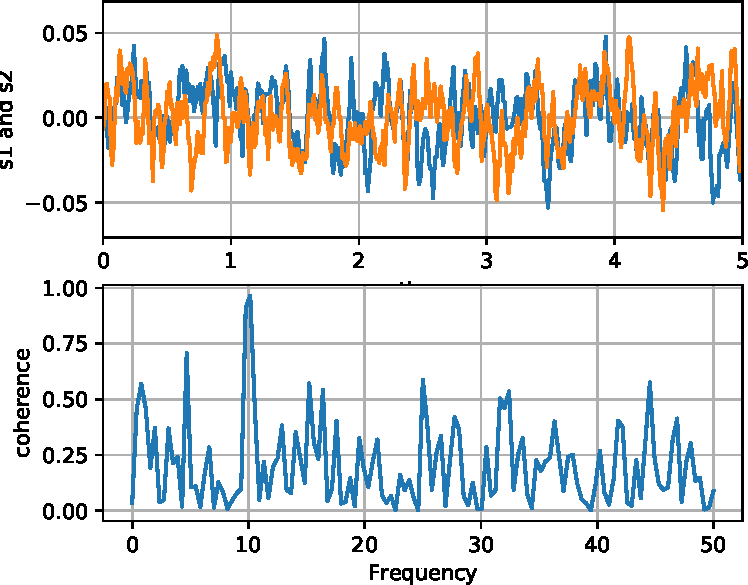
\includegraphics[width=.3\textwidth]{demo1.pdf}\hfill
	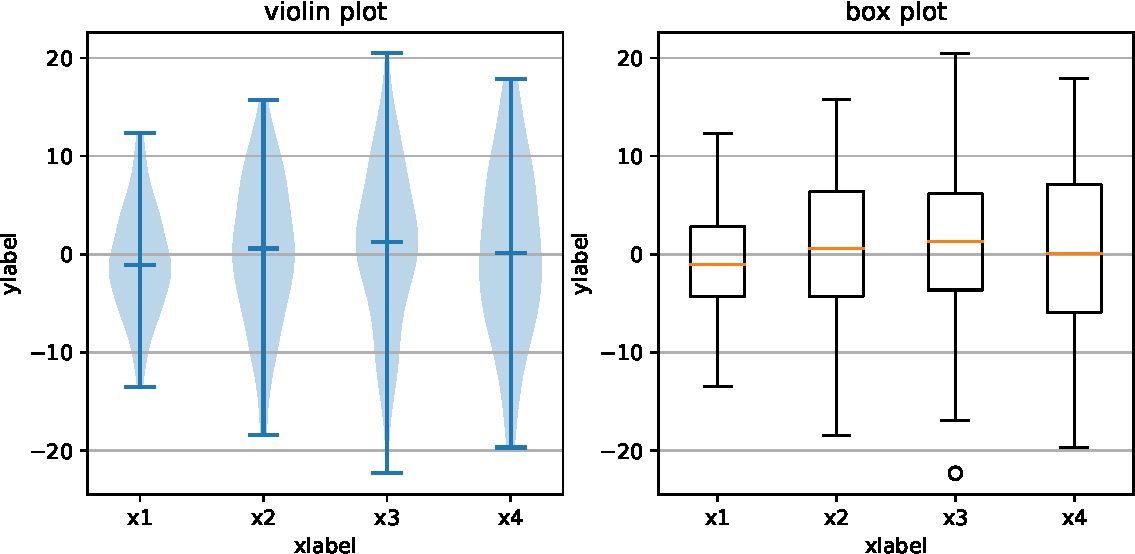
\includegraphics[width=.42\textwidth]{demo5.pdf}\hfill
	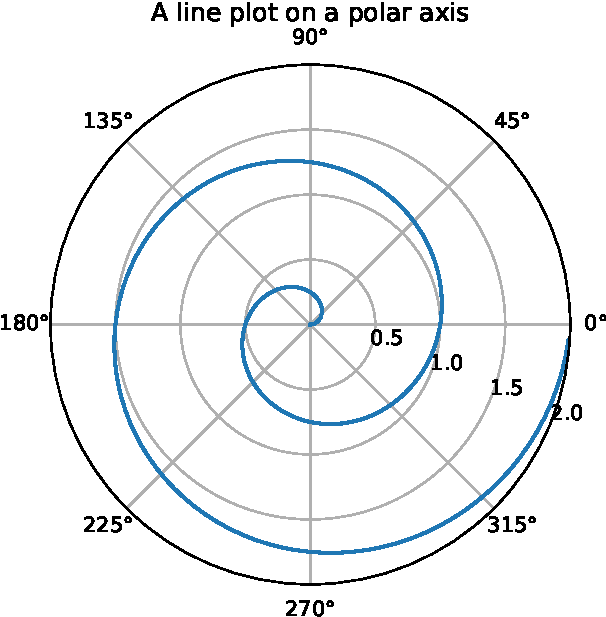
\includegraphics[width=.22\textwidth]{demo3.pdf}\\
	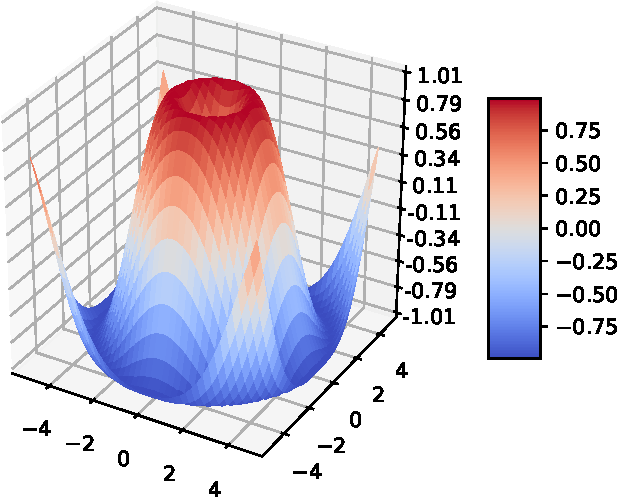
\includegraphics[width=.32\textwidth]{demo4.pdf}\hfill
	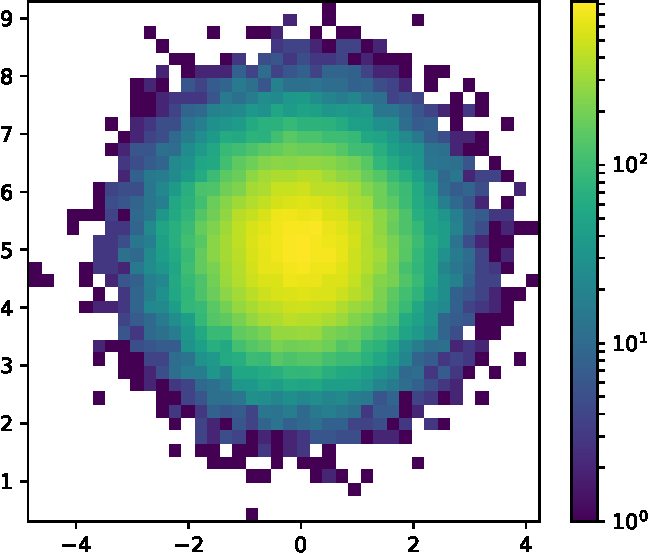
\includegraphics[width=.28\textwidth]{demo2.pdf}\hfill
	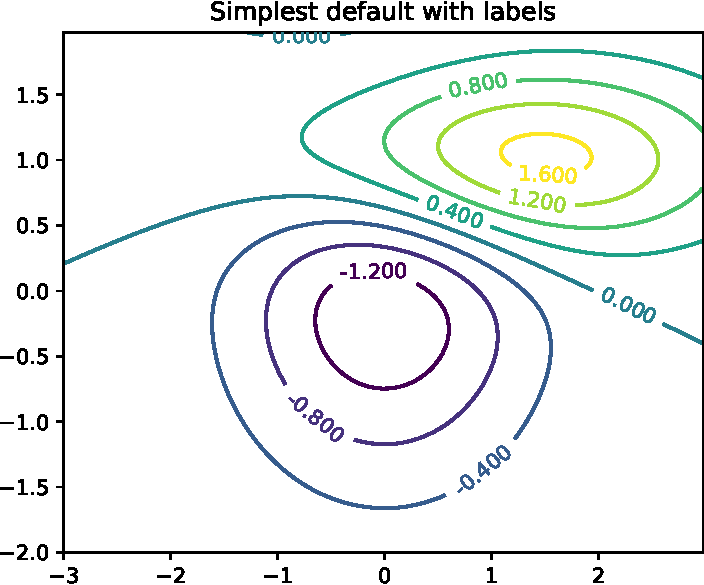
\includegraphics[width=.3\textwidth]{demo6.pdf}
\end{center}
\end{frame}

%=============================================================================%
%=============================================================================%
\begin{frame}{Anatomy of a figure}

\begin{center}
	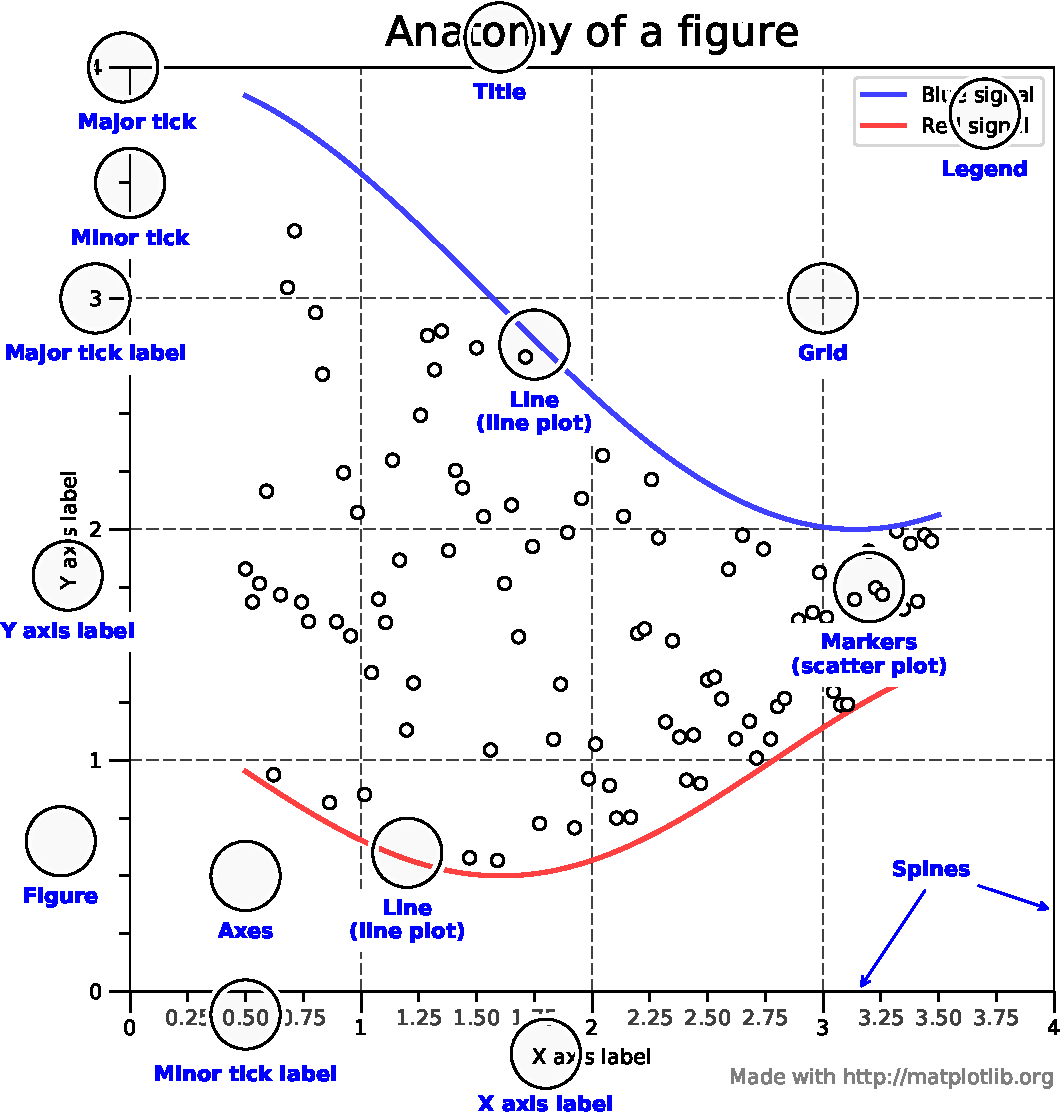
\includegraphics[width=.6\textwidth]{anatomy_figure.pdf}
\end{center}
\end{frame}

%=============================================================================%
%=============================================================================%
\begin{frame}[fragile]
\frametitle{My first plot}

\begin{lstlisting}[style=python]
import numpy as np
import matplotlib.pyplot as plt

# Generate sinusoidal data
x = np.linspace(0, 4*np.pi, 100)
y = np.sin(x)

# Plot sinusoidal curve
plt.plot(x, y, color="blue")
plt.xlabel("Time")
plt.ylabel("Amplitude")
plt.title("My first Python plot")
\end{lstlisting}

\vspace{-0.5cm}
\begin{center}
	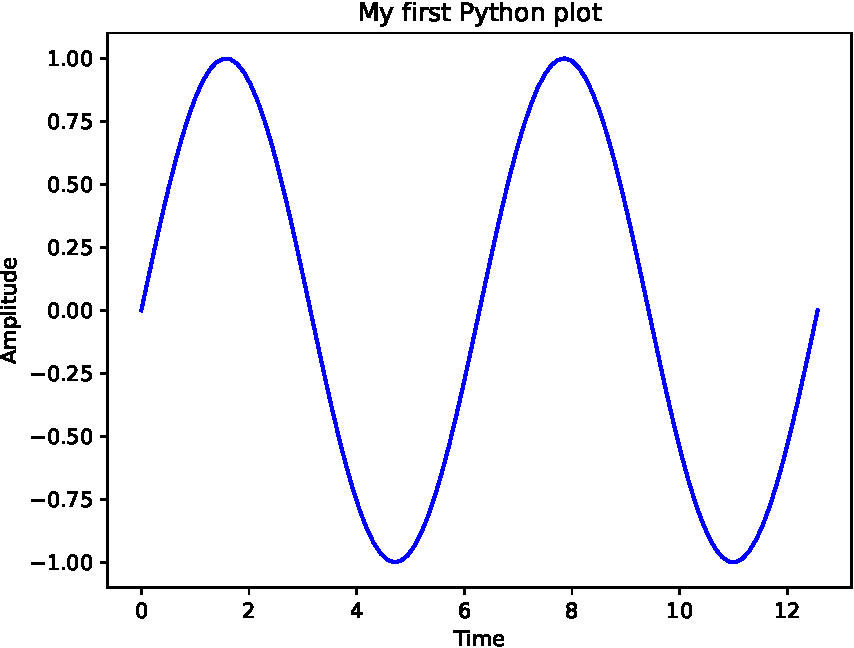
\includegraphics[width=.35\textwidth]{plot1.pdf}
\end{center}

\end{frame}

%=============================================================================%
%=============================================================================%
\begin{frame}[fragile]
\frametitle{Subplots}

\begin{lstlisting}[style=python]
plt.subplot(2, 1, 1) # 2 rows, 1 column, first plot
plt.plot(x, np.sin(x), color="b", label="Sine")
plt.ylabel("Amplitude")
plt.legend(loc="upper right")

plt.subplot(2, 1, 2) # 2 rows, 1 column, second plot
plt.plot(x, np.cos(x), color="r", label="Cosine")
plt.xlabel("Time")
plt.ylabel("Amplitude")
plt.legend(loc="upper right")
\end{lstlisting}

\vspace{-0.5cm}
\begin{center}
	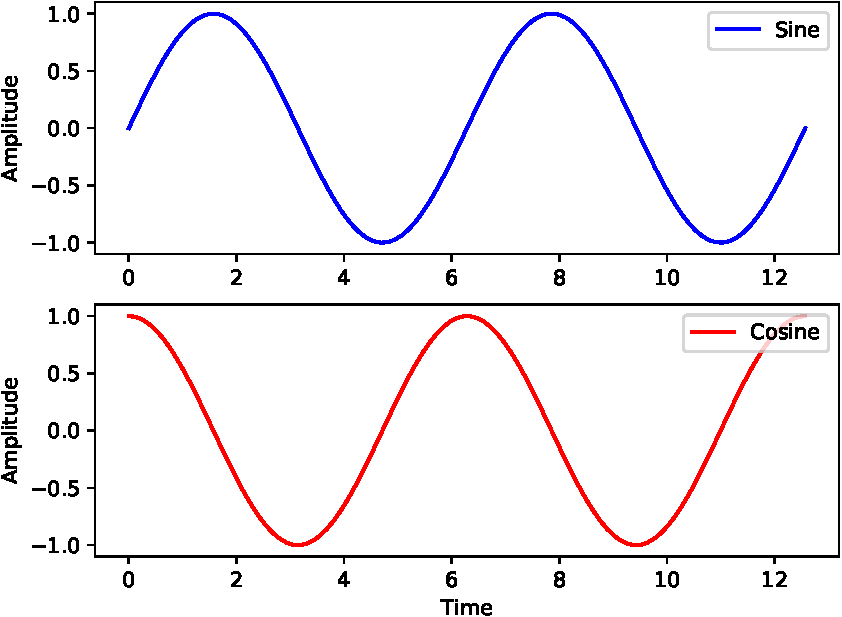
\includegraphics[width=.4\textwidth]{plot2.pdf}
\end{center}

\end{frame}

%=============================================================================%
%=============================================================================%
\begin{frame}[fragile]
\frametitle{Histograms}

\begin{lstlisting}[style=python]
# Generate 1000 normally distributed numbers
x1 = np.random.randn(1000) 
x2 = np.random.randn(1000) 

# 1D histogram (x1)
plt.subplot(1, 2, 1)
plt.hist(x1, bins=20)

# 2D histogram (x1 vs x2)
plt.subplot(1, 2, 2)
plt.hist2d(x1, x2, bins=20)
plt.colorbar()
\end{lstlisting}

\vspace{-0.6cm}
\begin{center}
	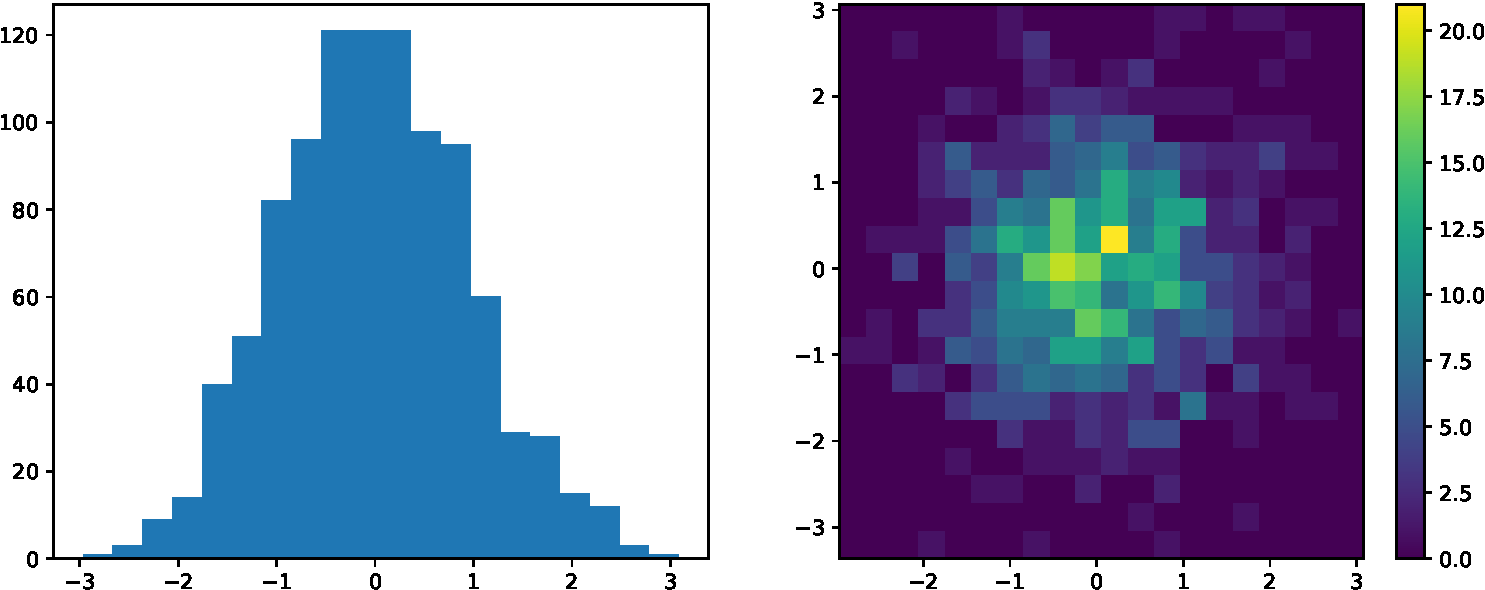
\includegraphics[width=.72\textwidth]{plot3.pdf}
\end{center}

\end{frame}

%=============================================================================%
%=============================================================================%
\begin{frame}[fragile]
\frametitle{Boxplots and violin plots}

\begin{lstlisting}[style=python]
# Generate four sets of random numbers
data = [np.random.randn(1000) for i in range(4)]

# Boxplot
plt.subplot(1, 2, 1)
plt.boxplot(data)

# Violin plot
plt.subplot(1, 2, 2)
plt.violinplot(data)
\end{lstlisting}

\vspace{-0.6cm}
\begin{center}
	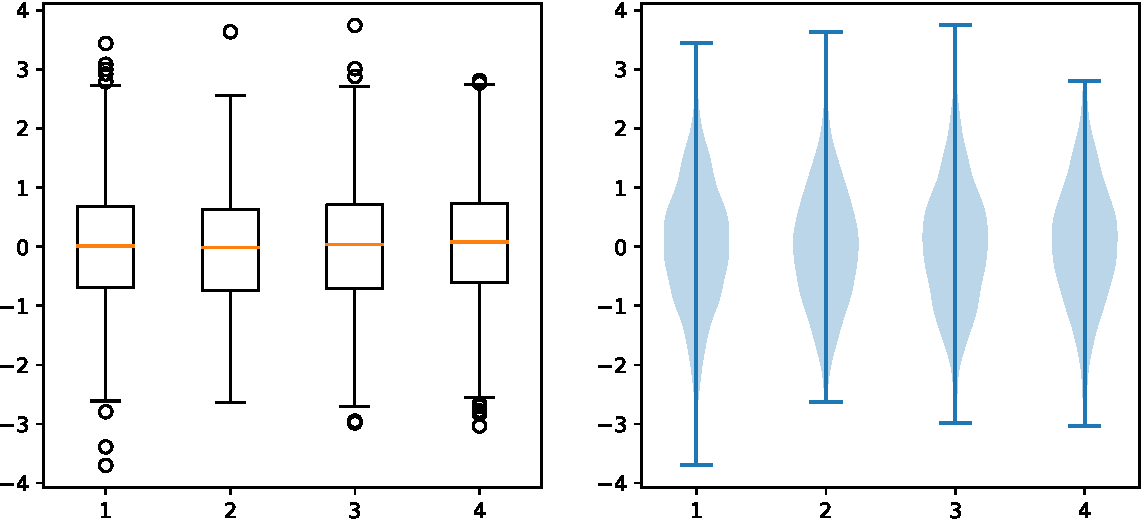
\includegraphics[width=.72\textwidth]{plot4.pdf}
\end{center}

\end{frame}

%=============================================================================%
%=============================================================================%
\begin{frame}[fragile]
\frametitle{Contour plot}

\tiny
\begin{lstlisting}[style=python]
# import |\href{https://matplotlib.org/tutorials/colors/colormaps.html}{colormaps}|
from matplotlib import cm

# Generate some x, y, z data
x = np.arange(-2.5, 2.5, 0.1)
y = np.arange(-2.5, 2.5, 0.1)
x, y = np.meshgrid(x, y) 
z = np.exp(-x**2 - y**2)

# Contour plot
plt.contourf(x, y, z, cmap=cm.inferno)
plt.colorbar()
\end{lstlisting}

\vspace{-0.8cm}
\begin{center}
	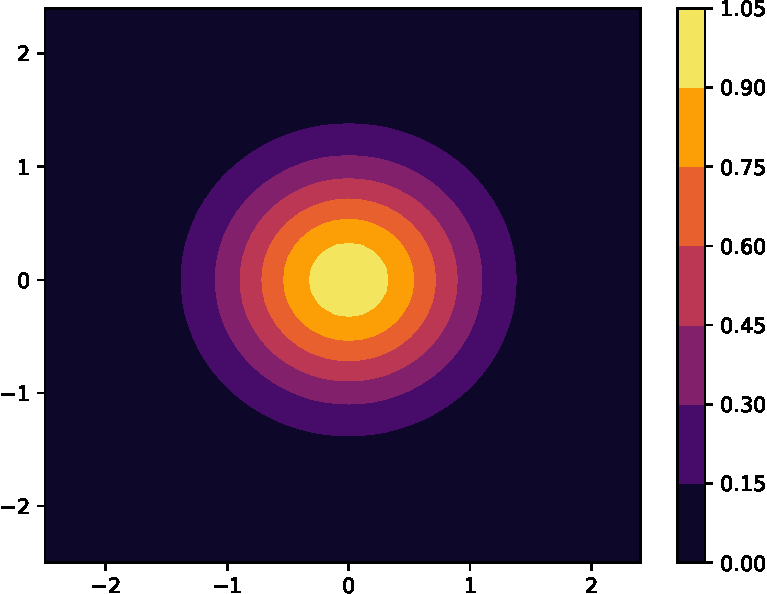
\includegraphics[width=.42\textwidth]{plot5.pdf}
\end{center}

\end{frame}


\begin{frame}[fragile]
\frametitle{Working with data and matplotlib}
\begin{itemize}%\addtolength{\itemsep}{-0.5\baselineskip}
    \item Typical structure of 3D data 
\begin{center}
    { \ttfamily
    \begin{tabular}{|l|l|l|}\hline
        column\_x & column\_y & column\_z \\ \hline
        0.897238 & 100000 & 4.06333241929155 \\
        0.916328 & 500 & 5.1788870872331 \\
        0.954509 & 100909 & 5.1788870872331 \\
        .... & ... & ... \\ \hline
    \end{tabular}
    } 
\end{center}
    \item  Data needs to be transformed to a pivot table before plotting. Example:
\begin{lstlisting}[style=pythonsmall]
print(z)
# [[3.72665317e-06 6.08307642e-06 9.73288695e-06 ... 1.52642052e-05
#   9.73288695e-06 6.08307642e-06]
#  ...
#  [6.08307642e-06 9.92950431e-06 1.58871492e-05 ... 2.49160097e-05
#   1.58871492e-05 9.92950431e-06]]
\end{lstlisting} \pause \vspace{-20pt}
    \item Transform to pivot table with \href{https://pandas.pydata.org/pandas-docs/stable/reference/api/pandas.pivot_table.html}{\texttt{pandas.pivot\_table()}} (see later)
\end{itemize}
\end{frame}

%=============================================================================%
\begin{frame}[fragile]
\frametitle{3D surface}

\tiny
\begin{lstlisting}[style=python]
from mpl_toolkits.mplot3d import Axes3D

# Create figure amenable for 3D plotting
hFig = plt.figure()
hAx = hFig.gca(projection="3d")

# Plot the surface
hSurf = hAx.plot_surface(x, y, z, cmap=cm.inferno)
plt.colorbar(hSurf, shrink=0.5)
\end{lstlisting}

\vspace{-0.8cm}
\begin{center}
	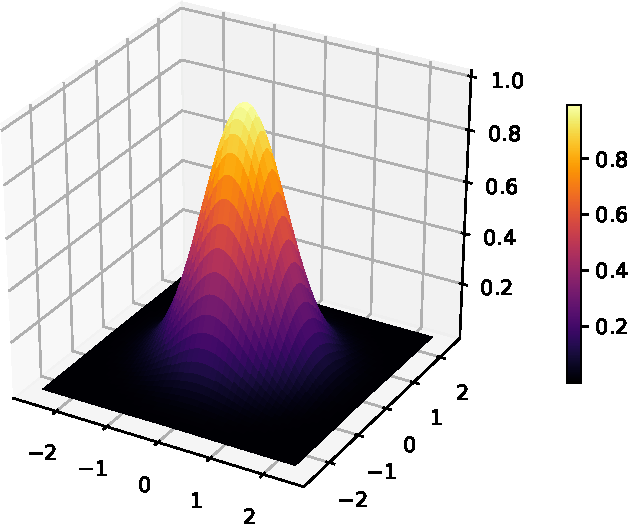
\includegraphics[width=.42\textwidth]{plot6.pdf}
\end{center}

\end{frame}

\begin{frame}[fragile]
\frametitle{Mathematical annotations in graphs}
    \begin{itemize}
        \item Broad support for \href{https://matplotlib.org/users/text_intro.html}{text} annotation in matplotlib
    \end{itemize}
\begin{center}
	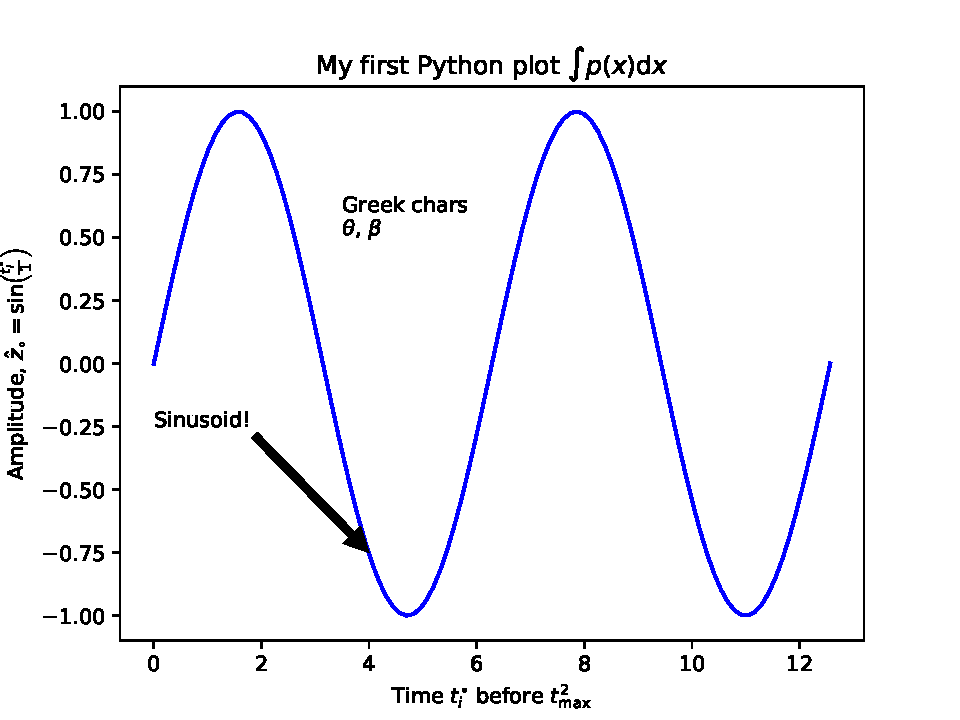
\includegraphics[width=0.8\textwidth]{plot_text_annotate.pdf}
\end{center}
\end{frame}
            
            
\begin{frame}[fragile]
    \tiny
\frametitle{Mathematical annotations in graphs}
            \begin{lstlisting}[style=python]
# Generate sinusoidal data
x = np.linspace(0, 4*np.pi, 100)
y = np.sin(x)

# Plot sinusoidal curve
plt.plot(x, y, color="blue")

# labels using latex commands 
plt.xlabel(r"Time $t_{i}^{\bullet}$ before $t_{\mathrm{max}}^{2}$")
plt.ylabel(r"Amplitude, $\hat{z}_{\circ} = \sin \left(\frac{t_{i}^{\bullet}}{1} \right)$")

# plot title
plt.title(r"My first Python plot $\int p(x) \mathrm{d}x$") 

# text label with arrow using| \href{https://matplotlib.org/api/_as_gen/matplotlib.pyplot.annotate.html?highlight=pyplot%20annotate#matplotlib-pyplot-annotate}{pyplot.annotate} | 
plt.annotate(s = "Sinusoid!", xy=(4.0, -0.75), xytext=(0,-0.25), arrowprops=dict(facecolor="black",linewidth=0.01))

# text annotation within the plot using| \href{https://matplotlib.org/api/_as_gen/matplotlib.pyplot.text.html?highlight=pyplot%20text#matplotlib.pyplot.text}{pyplot.text} |
plt.text(x=4.7, y = 0.5, s = r"A label $\theta$, $\beta$")
\end{lstlisting}
\end{frame}
    

\begin{frame}[fragile]
\frametitle{Saving figures to files}
    \begin{itemize}
        \item One can automate saving figures to files using \href{https://matplotlib.org/api/_as_gen/matplotlib.pyplot.savefig.html?highlight=pyplot%20savefig#matplotlib.pyplot.savefig}{pyplot.savefig}
\begin{lstlisting}[style=python]
# at the end of the figure

# store figure in file (png, eps, pdf, svg, etc)
plt.savefig(fname="lineplot.svg")
plt.close() # plot stays in memory unless closed
\end{lstlisting}
        \item Note that svg format can easily be edited using vector graphics software like Illustrator or Inkscape
    \end{itemize}
\end{frame}

\begin{frame}[fragile]
    \frametitle{Finer control over multipanel figures using \texttt{gridspec}}
    \begin{lstlisting}[style=pythonsmall]
import matplotlib.gridspec as gridspec

# set up a 2 x 2 grid with lower row half the size of top row
gs = gridspec.GridSpec(
        nrows=2
        ,ncols=2
        ,height_ratios=[1,0.5]
        ,width_ratios=[1,1])

plt.figure()
# first subplot top left corner, return Axes object for control over axes
ax = plt.subplot(gs[0,0])
ax.plot(...)

# work with axes, e.g., remove x-tick labels
ax.set_xticklabels([])
 
# second subplot top right corner
plt.subplot(gs[0,1])
plt.plot(...)

# third subplot bottom left corner
plt.subplot(gs[1,0])
plt.plot(...)
 
# second subplot bottom right corner
plt.subplot(gs[0,1])
plt.plot(...)

plt.show()
    \end{lstlisting}
\end{frame}
%=============================================================================%
%=============================================================================%
% End of Document
%=============================================================================%
%=============================================================================%
\end{document}
